\section{Zasady działania kompasu. Zofia Sosińska}\label{chap:naw}

Projekt kompasu jest na tyle prosty, aby nie przytłoczyć gracza nadmierną liczba bodźców. Składa się horyzontalnego, jednolitego paska, na którym wyświetlane będą informacje, symbolu ośmiokąta, wskazującego na przestrzeń znajdującą się centralnie przed bohaterem, oraz z bocznych pasków, wyróżniających końce narzędzia.

\begin{figure}[htbp]
    \centering
    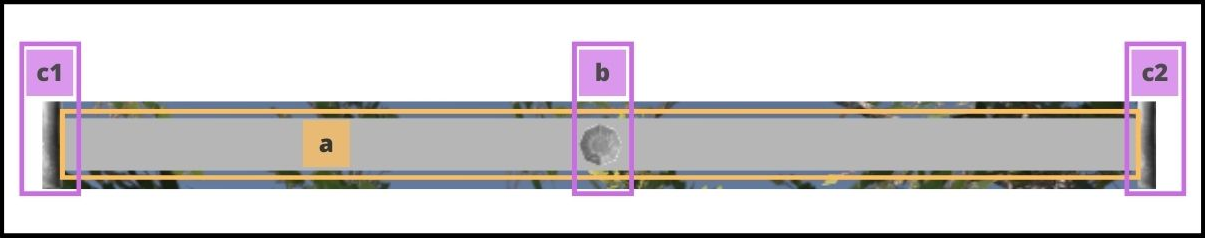
\includegraphics[width=0.9\textwidth]{images/ui/opis_ekementow_kompasu.png}
    \caption{Rozpiska elementów: a. główny pasek, b. symbol środka, c1., c2. paski końców kompasu.}\label{fig:compass_design}
\end{figure}

\begin{lstlisting}[caption=Fragment kodu odpowiedzialny za ustawienie symbolu na pasku kompasu]

void SetMarkerPosition(RectTransform markerTransform, Vector3 worldPosition)
    {
        Vector3 dirToTarget = worldPosition - CameraTransform.position;
        float angle = Vector2.SignedAngle(new Vector2(dirToTarget.x, dirToTarget.z), new Vector2(CameraTransform.transform.forward.x, CameraTransform.transform.forward.z));
        float compassPositionX = Mathf.Clamp(2 * angle / Camera.main.fieldOfView, -1, 1);
        if (compassPositionX == 1 || compassPositionX == (-1))
        {
            markerTransform.anchoredPosition = new Vector2(0, 100);
        }
        else
        {
            markerTransform.anchoredPosition = new Vector2(compassBarTransform.rect.width / 2 * compassPositionX, 0);
        }
    }
\end{lstlisting}